\documentclass[12pt,a4paper]{article}
\usepackage[utf8]{inputenc} % inutile avec XeLaTeX/LuaLaTeX
\usepackage[T1]{fontenc}
\usepackage{amsmath,amssymb,mathrsfs,tikz,times,pifont}
\usepackage{amsfonts}
\usepackage{systeme}
\usepackage{tkz-tab}
\usepackage{tikz}
\usepackage{pgfplots}
\pgfplotsset{compat=1.15}
\usepackage{enumitem}
\usepackage{multicol}
\usepackage{lmodern}
\newcommand\circitem[1]{%
\tikz[baseline=(char.base)]{
\node[circle,draw=gray, fill=red!55,
minimum size=1.2em,inner sep=0] (char) {#1};}}
\newcommand\boxitem[1]{%
\tikz[baseline=(char.base)]{
\node[fill=cyan,
minimum size=1.2em,inner sep=0] (char) {#1};}}
\setlist[enumerate,1]{label=\protect\circitem{\arabic*}}
\setlist[enumerate,2]{label=\protect\boxitem{\alph*}}
\everymath{\displaystyle}
\usepackage[left=1cm,right=1cm,top=1cm,bottom=1.7cm]{geometry}
\usepackage[colorlinks=true, linkcolor=blue, urlcolor=blue, citecolor=blue]{hyperref}
\usepackage{array,multirow}
\usepackage[most]{tcolorbox}
\usepackage{varwidth}
\usepackage{float}
\tcbuselibrary{skins,hooks}
\usetikzlibrary{patterns}

\newtcolorbox{exa}[2][]{enhanced,breakable,before skip=2mm,after skip=5mm,
colback=yellow!20!white,colframe=black!20!blue,boxrule=0.5mm,
attach boxed title to top left ={xshift=0.6cm,yshift*=1mm-\tcboxedtitleheight},
fonttitle=\bfseries,
title={#2},#1,
boxed title style={frame code={
\path[fill=tcbcolback!30!black]
([yshift=-1mm,xshift=-1mm]frame.north west)
arc[start angle=0,end angle=180,radius=1mm]
([yshift=-1mm,xshift=1mm]frame.north east)
arc[start angle=180,end angle=0,radius=1mm];
\path[left color=tcbcolback!60!black,right color = tcbcolback!60!black,
middle color = tcbcolback!80!black]
([xshift=-2mm]frame.north west) -- ([xshift=2mm]frame.north east)
[rounded corners=1mm]-- ([xshift=1mm,yshift=-1mm]frame.north east)
-- (frame.south east) -- (frame.south west)
-- ([xshift=-1mm,yshift=-1mm]frame.north west)
[sharp corners]-- cycle;
},interior engine=empty,
},interior style={top color=yellow!5}}

\usepackage{fancyhdr}
\usepackage{eso-pic}
\usepackage{tkz-tab}
\AddToShipoutPicture{
    \AtTextCenter{%
        \makebox[0pt]{\rotatebox{80}{\textcolor[gray]{0.7}{\fontsize{5cm}{5cm}\selectfont PGB}}}
    }
}

\usepackage{verbatim}

\usepackage{color,soul}
\usetikzlibrary{arrows}
\newcounter{exemple} % Compteur pour les questions

% Définir la commande pour afficher une question numérotée
\newcommand{\exemple}{%
  \refstepcounter{exemple}%
  \textbf{\textcolor{green}{Exemple \theexemple :}} \ignorespaces
}
%---------------------------------------
\definecolor{myorange}{rgb}{1.0, 0.8, 0.0}

% Définir un compteur pour les exercices d'application
\newcounter{exerciceapp}

% Définir la commande pour afficher un exercice d'application numéroté
\newcommand{\exerciceapp}{%
  \refstepcounter{exerciceapp}%
  \textbf{\textcolor{myorange}{Exercice d'application \theexerciceapp :}} \ignorespaces
}
%--------------------------------------
% Définir un compteur pour les exercices d'application
\newcounter{correction}

% Définir la commande pour afficher un correction exercice d'application numéroté
\newcommand{\correction}{%
  \refstepcounter{correction}%
  \textbf{\textcolor{myorange}{Correction \thecorrection :}} \ignorespaces
}
%--------------------------------------
% Commande pour ajouter du texte en arrière-plan
\usepackage{fancyhdr}
\usepackage{eso-pic}
%\usepackage{tkz-tab}
\AddToShipoutPicture{
    \AtTextCenter{%
        \makebox[0pt]{\rotatebox{80}{\textcolor[gray]{0.7}{\fontsize{5cm}{5cm}\selectfont PGB}}}
    }
}
%This command takes a colour as an optional argument; the default colour is black.
\usetikzlibrary{shapes.geometric,fit}
\newcommand{\myul}[2][black]{\setulcolor{#1}\ul{#2}\setulcolor{black}}
\newcommand\tab[1][1cm]{\hspace*{#1}}

\begin{document}
% En-tête personnalisée
\begin{center}
    \Large\textbf{\underline{\textcolor{red}{Fonction logarithme Népérien}}}\\[-0.1cm]
    \normalsize\textbf{Prof : M. BA} \hfill \textbf{Classe : TS2}\\[-0.1cm]
    \textbf{Année scolaire : 2025 -- 2026}
\end{center}


\section*{\underline{\textbf{\textcolor{red}{Introduction :}}}}

En 1614, un mathématicien écossais, John Napier (1550 ; 1617) ci-contre, plus connu sous le nom francisé de Neper publie « Mirifici logarithmorum canonis descriptio ».
Dans cet ouvrage, qui est la finalité d’un travail de 20 ans, Neper présente un outil permettant de simplifier les calculs opératoires : le logarithme.
Neper construit le mot à partir des mots grecs « logos » (logique) et arithmos (nombre).
Toutefois cet outil ne trouvera son essor qu’après la mort de Neper. Les mathématiciens anglais Henri Briggs (1561 ; 1630) et William Oughtred (1574 ; 1660) reprennent et prolongent les travaux de Neper.
Les mathématiciens de l’époque établissent alors des tables de logarithmes de plus en plus précises.
L’intérêt d’établir ces tables logarithmiques est de permettre de substituer une multiplication par une addition (paragraphe II). Ceci peut paraître dérisoire aujourd’hui, mais il faut comprendre qu’à cette époque, les calculatrices n’existent évidemment pas, les nombres décimaux ne sont pas d’usage courant et les opérations posées telles que nous les utilisons ne sont pas encore connues. Et pourtant l'astronomie, la navigation ou le commerce demandent d’effectuer des opérations de plus en plus complexes.

\section*{\underline{\textbf{\textcolor{red}{I.Définition et propriétés}}}}
\subsection*{\underline{\textbf{\textcolor{red}{1.Définition}}}}
On appelle fonction logarithmique népérien la fonction notée $\ln$ qui est définie sur $]0\;;\ +\infty[$ et qui vérifie $(\ln (x))'=\dfrac{1}{x}\ $ et $\ \ln 1=0$

$$\begin{array}{rcl}
\ln\ :\ ]0\;;\ +\infty[ & \longrightarrow & \mathbb{R} \\
x & \longmapsto & \ln x
\end{array}$$
\subsection*{\underline{\textbf{\textcolor{red}{2.Conséquences de la définition}}}}
Soit $u$ une fonction définie sur un intervalle $I$ de $\mathbb{R}$ alors :

- $\ln u$ existe si $u > 0$

- $\ln |u|$ existe si $u \neq 0$

- $\ln u^{2}$ existe si $u \neq 0$

\subsection*{\underline{\textbf{\textcolor{red}{3.Propriétés}}}}
Les propriétés fondamentales de la fonction logarithmique, $\ln$, sont :
\begin{itemize}
    \item 
    \(
    \ln(ab) = \ln a + \ln b \quad \text{pour } a > 0 \text{ et } b > 0.
    \)
    \item 
    \(
    \ln\left(\dfrac{a}{b}\right) = \ln a - \ln b \quad \text{pour } a > 0 \text{ et } b > 0.
    \)
    \item 
    \(
    \ln(a^p) = p \ln a \quad \text{pour } a > 0 \text{ et } p \in \mathbb{R}.
    \)
    \item 
    \(
    \ln\sqrt{a} = \dfrac{1}{2} \ln a \quad \text{pour } a > 0.
    \)
\end{itemize}

\subsection*{\underline{\textbf{\textcolor{red}{4.Remarque}}}}
La fonction $\ln$ est strictement croissante sur son domaine $]0\;;\ +\infty[$, c'est-à-dire que :
\[
\forall a, b \in ]0\;;\ +\infty[, \quad a < b \implies \ln a < \ln b.
\]

\section*{\underline{\textbf{\textcolor{red}{II.Limites et Dérivée}}}}

\subsection*{\underline{\textbf{\textcolor{red}{1.Limites aux bornes de $D_{ln}$}}}}
\begin{itemize}
    \item $\lim_{x \to 0^+} \ln x = -\infty$.
    \item $\lim_{x \to +\infty} \ln x = +\infty$.
\end{itemize}
\subsection*{\underline{\textbf{\textcolor{red}{2.Limites usuelles}}}}
\begin{itemize}
    \item $\lim_{x \to 0^+} x \ln x = 0$.
    \item $ \lim_{x \to +\infty} \frac{\ln x}{x} = 0 $
    \item $\lim_{{x \to 0}} \frac{\ln(x+1)}{x}=1$\\
Soit a un nombre rationnel strictement positif.
   \item $\lim_{{x \to 0^+}} x^{\alpha}\ln(x) = 0^{-} $
   \item $\lim_{{x \to +\infty}} \frac{\ln(x)}{x^{\alpha}}=0^{+}$
\end{itemize}
\paragraph{ Croissances comparées :}
Soit $\alpha$ un nombre réel strictement positif ($\alpha > 0$). 
Au voisinage de $0^+$ et de $+\infty$, la fonction puissance l'emporte sur la fonction logarithme népérien :

\begin{itemize}
    \item \textbf{En $0^+$ :} 
    \(
    \lim\limits_{x \to 0^+} x \ln x = 0 \quad \text{et plus généralement,} \quad \lim\limits_{x \to 0^+} x^{\alpha} \ln x = 0^{-}
    \)
    
    \item \textbf{En $+\infty$ :} 
    \(
    \lim\limits_{x \to +\infty} \frac{\ln x}{x} = 0 \quad \text{et plus généralement,} \quad \lim\limits_{x \to +\infty} \frac{\ln x}{x^{\alpha}} = 0^{+}
    \)
\end{itemize}
\underline{\textbf{\textcolor{red}{Preuve de quelques limites}}}\\
Montrons que $\lim_{{x \to 0^+}} x^{\alpha}\ln(x) = 0^{-}$ pour $\alpha=1$\\
pour tout $x\in]0;+\infty[,$ en posant $X=\frac{1}{x}$, on a : $xlnx=-\frac{lnX}{X}$\\
ainsi, $\lim_{{x \to 0^{+}}} -\frac{\ln(X)}{X}=0^{-}$
Donc $\lim_{{x \to 0^+}} x^{\alpha}\ln(x) = 0^{-}$\\
\underline{\textbf{\textcolor{red}{Exemple}}}\\

Déterminer les limites suivantes:
\begin{enumerate}
\item \( \lim\limits_{x \to +\infty} x\ln(x)-x^{2}+1\)

\item \( \lim\limits_{x \to 0} x\ln(x)-x^{2}+1\)

\item \( \lim\limits_{x \to +\infty} \frac{x\ln(x)}{x^{2}+1}\)
\end{enumerate}

\underline{\textbf{\textcolor{red}{Exercice d'application}}}\\
Déterminer les limites suivantes:

\begin{enumerate}
\item \( \lim\limits_{x \to +\infty} x+1-\ln(x)\)

\item \( \lim\limits_{x \to +\infty} \frac{x}{2}[\ln(1+\frac{1}{x})] \)

\item \( \lim\limits_{x \to +\infty} \frac{\ln(x)}{\sqrt{x}} \)

\item \( \lim\limits_{x \to 1^{+}} (x-1)\ln(x-1) \)

\item \( \lim\limits_{x \to 1^{+}} \frac{x}{x+1}-\ln(x+1) \)
\end{enumerate}

\subsection*{\underline{\textbf{\textcolor{red}{3.Limites des composées avec ln}}}}
Soit $U(x)$ une fonction strictement positive.\\
Cherchons $\lim_{{x \to a}} \ln[u(x)]$\\

$\textbf{Si}
 \begin{cases}
 \lim\limits_{{x \to a}} u(x)=l\\[2mm]
 \lim\limits_{{X \to l}} \ln(X)=l'
 \end{cases} \implies \lim\limits_{{x \to a}} \ln[u(x)]=l'
$

\underline{\textbf{\textcolor{red}{Exemple}}}\\
Calcule la limite suivante\\
$\displaystyle \lim\limits_{x \to +\infty} \ln\left(\frac{x^2}{2x^2 - 1}\right)$

\underline{\textbf{\textcolor{red}{Solution}}}\\

\textbf{Étape 1 : Limite de la fonction rationnelle à l'intérieur du logarithme}\\
Quand $x \to +\infty$, le comportement en $+\infty$ d'une fonction rationnelle est donné par le rapport
                de ses termes de plus haut degré :
                
                $
                \displaystyle
                \begin{aligned}
                \lim\limits_{x \to +\infty} \frac{x^2}{2x^2 - 1} &= \lim_{x \to +\infty} \frac{x^2}{2x^2}\\ 
                                                                 &= \frac{1}{2}
                \end{aligned}
                $

\textbf{Étape 2 : Application du théorème de composition des limites}\\
On pose $u(x) = \dfrac{x^2}{2x^2 - 1}$. 

\[
\text{Si }
\begin{cases}
\lim\limits_{x \to +\infty} u(x) = \dfrac{1}{2} \\[2mm]
\lim\limits_{X \to \frac{1}{2}} \ln(X) = \ln\left(\dfrac{1}{2}\right)
\end{cases}
\text{ alors } \lim_{x \to +\infty} \ln\left[u(x)\right] = \ln\left(\frac{1}{2}\right)
\]

\textbf{Étape 3 : Simplification du résultat}\\
En utilisant la propriété $\ln\left(\frac{1}{a}\right) = -\ln(a)$, on obtient :
                $\ln\left(\frac{1}{2}\right) = -\ln(2)$

\textbf{Conclusion :}
$\displaystyle \lim\limits_{x \to +\infty} \ln\left(\frac{x^2}{2x^2 - 1}\right) = -\ln(2)$

\subsection*{\underline{\textbf{\textcolor{red}{II. Dérivée et dérivée de la composée}}}}

Soient $u$ et $v$ deux fonctions dérivables et strictement positives sur un intervalle $I$ de $\mathbb{R}$.

\begin{itemize}
    \item \textbf{Dérivée de $\ln(u)$ :}
    \(
    \big[\ln(u(x))\big]' = \frac{u'(x)}{u(x)}
    \)

    \item \textbf{Dérivée de $\ln\left(\frac{u}{v}\right)$ :}
    \(
    \left[\ln\left(\frac{u(x)}{v(x)}\right)\right]' = \left[\ln(u(x)) - \ln(v(x))\right]' = \frac{u'(x)}{u(x)} - \frac{v'(x)}{v(x)}
    \)
\end{itemize}

\paragraph{\textcolor{red}{Exemples :}}
Déterminer la fonction dérivée de chacune des fonctions suivantes :

\begin{enumerate}
    \item $f(x) = \frac{\ln(x^{2}+2x+9)}{x} \quad \text{sur } \mathbb{R}^*$ 
    \quad \textit{(Forme $\frac{u}{v}$ combinée avec $\ln$)}
    
    \item $g(x) = \ln\left(\frac{x^{2}+2x+9}{x-2}\right) \quad \text{sur } ]2 \;;\ +\infty[$
\end{enumerate}
\section*{\underline{\textbf{\textcolor{red}{III.Etude le fonction ln}}}}
Soit $f$ la fonction définie par $f(x) = \ln(x)$.

\paragraph{Domaine de définition $D_{f}$ :}
$f(x)$ existe si et seulement si $x \in \mathbb{R}^*_+$. 
Ainsi, le domaine de définition est :
\[
D_{f} = \mathbb{R}^*_+ = ]0\,;\,+\infty[
\]

\subsection*{\underline{\textbf{\textcolor{red}{1. Limites aux bornes de $D_{f}$}}}}

\paragraph{En $0^+$ :}
\(
\lim_{x \to 0^+} \ln(x) = -\infty
\)
\textit{(La droite d'équation $x = 0$ est asymptote verticale à la courbe $\mathcal{C}_f$.)}

\paragraph{En $+\infty$ :}
\(
\lim_{x \to +\infty} \ln(x) = +\infty
\)

\subsection*{\underline{\textbf{\textcolor{red}{2. Dérivée et sens de variation}}}}

Pour tout $x \in ]0\,;\,+\infty[$, $f$ est dérivable et :
\(
f'(x) = \frac{1}{x}
\)

Pour tout $x \in ]0\,;\,+\infty[$, $f'(x) > 0$. On en déduit que la fonction $f$ est \textbf{strictement croissante} sur $]0\,;\,+\infty[$.

\underline{Tableau de variation}

% ==============================================================================
% NOTE TECHNIQUE / BUG ENCONTRE AVEC TKZ-TAB :
% ------------------------------------------------------------------------------
% Pourquoi nous utilisons du TikZ pur au lieu de \tkzTabInit / \tkzTabVal ici :
%
% 1. Conflit R/ + \tkzTabVal + Double barre (-D/) :
%    Lorsqu'une flèche de variation est continue avec l'option 'R/' (Repeat)
%    et démarre sur une double barre, tkz-tab ne crée qu'un seul nœud interne (FR12).
%
% 2. Plantage des nœuds internes :
%    Appeler \tkzTabVal[draw]{2}{3}{...} sur la seconde portion d'intervalle 
%    déclenche une erreur fatale ("No shape named 'FR22' is known") car la
%    seconde flèche n'existe pas en mémoire.
%
% 3. Bug d'affichage vertical :
%    Remplacer les indices par {1}{3} force l'affichage, mais dérègle les repères
%    verticaux de tkz-tab : la flèche traverse le tableau et la ligne de la dérivée.
%
% SOLUTION : Le tracé ci-dessous est réalisé en TikZ natif pour garantir un 
% positionnement parfait de la flèche, des pointillés et des valeurs (0 et 1).
% ==============================================================================

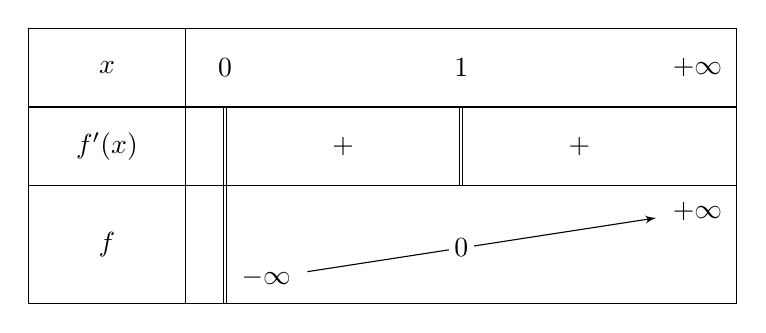
\begin{tikzpicture}
   \tkzTabInit{$x$ /1, $f'(x)$ /1, $f$ /1.5} {$0$ , $1$, $+\infty$}
   \tkzTabLine{d, +, d, +, } 
   \tkzTabVar{D- / $-\infty$, R/, + / $+\infty$}
   \tkzTabIma{1}{3}{2}{$0$}
   %\tkzTabIma{1}{3}{2}{$0$}
   %\tkzTabVal[draw]{2}{3}{0.3}{$e$}{$1$}
\end{tikzpicture}
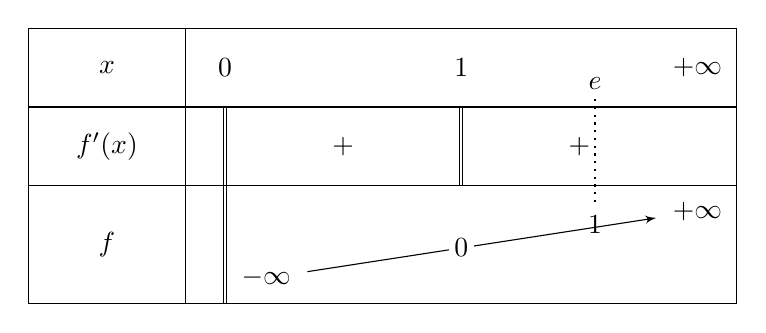
\begin{tikzpicture}
   \tkzTabInit{$x$ /1, $f'(x)$ /1, $f$ /1.5}
   {$0$ , $1$, $+\infty$}
   \tkzTabLine{d, +, d, +}
   \tkzTabVar{D-/$-\infty$, R/, +/$+\infty$}
   \tkzTabIma{1}{3}{2}{$0$}

\node (A) at (7.2,-0.7) {$e$};
\node (B) at (7.2,-2.5) {$1$};

\draw[dotted, thick] (A) -- (B);
\end{tikzpicture}
\subsection*{\underline{\textbf{\textcolor{red}{3.Branche infinie de ln}}}}
$\lim_{{x \to +\infty}} \frac{ln(x)}{x}=0$ donc ln admet une branche parabolique de direction (Ox) au voisinage de +$\infty$.\\

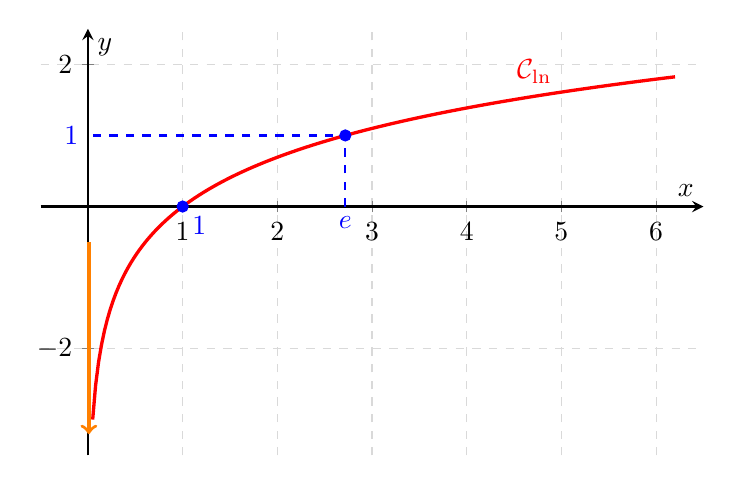
\begin{tikzpicture}
\begin{axis}[
    % Configuration des axes
    axis lines = middle,
    xlabel = {$x$},
    ylabel = {$y$},
    xmin = -0.5, xmax = 6.5,
    ymin = -3.5, ymax = 2.5,
    grid = major,
    grid style = {dashed, gray!30},
    width = 10cm, height = 7cm,
    samples = 200,
    domain = 0.05:6.2, % Domaine de tracé (légèrement supérieur à 0)
    enlargelimits = false,
    axis line style = {-stealth, thick}
]

    % Tracé de la courbe de ln(x)
    \addplot[very thick, red] {ln(x)};
    \node[red, above left] at (axis cs: 5, 1.6) {$\mathcal{C}_{\ln}$};

    % Points clés : (1, 0) et (e, 1)
    \addplot[only marks, mark=*, mark size=2pt, color=blue] coordinates {(1,0) (2.718,1)};
    
    % Traits pointillés pour f(e) = 1
    \draw[dashed, blue, thick] (axis cs: 2.718, 0) -- (axis cs: 2.718, 1) -- (axis cs: 0, 1);

    % Étiquettes des points remarquables
    \node[below right, blue] at (axis cs: 1, 0) {$1$};
    \node[below, blue] at (axis cs: 2.718, 0) {$e$};
    \node[left, blue] at (axis cs: 0, 1) {$1$};

    % Asymptote verticale x = 0 (axe des ordonnées)
    \draw[very thick, orange, ->] (axis cs: 0.01, -0.5) -- (axis cs: 0.01, -3.2);

\end{axis}
\end{tikzpicture}

\section*{\underline{\textbf{\textcolor{red}{IV. Application}}}}

\subsection*{\underline{\textbf{\textcolor{red}{1. Équations, inéquations et systèmes avec $\ln$}}}}

\subsubsection*{\underline{\textbf{\textcolor{red}{a°) Équations}}}}

Pour résoudre les équations comportant des logarithmes népériens, on peut procéder comme suit :
\begin{itemize}
    \item On détermine l'ensemble (ou domaine) de validité $D_v$.
    \item On utilise les propriétés algébriques pour se ramener à la forme $\ln(a) = \ln(b) \iff a = b$ (avec $a>0$ et $b>0$).
    \item On résout l'équation algébrique $a = b$.
    \item On conclut en ne retenant que les solutions qui appartiennent à $D_v$.
\end{itemize}

\paragraph{\underline{\textbf{\textcolor{red}{Exemple :}}}}
Résoudre dans $\mathbb{R}$ les équations suivantes :
\begin{enumerate}
    \item[a)] $\ln(x+1) = \ln(2x-1)$
    \item[b)] $\ln(x+1) - \ln(2x+1) = \ln(2x-1)$
\end{enumerate}

\paragraph{\underline{\textbf{\textcolor{blue}{Correction de l'exemple :}}}}
\begin{itemize}
    \item \textbf{Résolution de a) :} $\ln(x+1) = \ln(2x-1)$
    \begin{itemize}
        \item \textit{Domaine de validité $D_v$ :} 
        \[
        D_v = \{x \in \mathbb{R} \mid x+1 > 0 \text{ et } 2x-1 > 0\} = \left]-\frac{1}{2} \,;\, +\infty\right[ \cap \left]\frac{1}{2} \,;\, +\infty\right[ = \left]\frac{1}{2} \,;\, +\infty\right[
        \]
        \item \textit{Résolution :} Pour tout $x \in D_v$,
        \[
        \ln(x+1) = \ln(2x-1) \iff x+1 = 2x-1 \iff x = 2
        \]
        \item \textit{Conclusion :} $2 \in D_v$, donc $S = \{2\}$.
    \end{itemize}

    \item \textbf{Résolution de b) :} $\ln(x+1) - \ln(2x+1) = \ln(2x-1)$
    \begin{itemize}
        \item \textit{Domaine de validité $D_v$ :} $D_v = \left]\frac{1}{2} \,;\, +\infty\right[$.
        \item \textit{Résolution :} 
        \[
        \ln\left(\frac{x+1}{2x+1}\right) = \ln(2x-1) \iff \frac{x+1}{2x+1} = 2x-1 \iff x+1 = (2x-1)(2x+1)
        \]
        \[
        x+1 = 4x^2 - 1 \iff 4x^2 - x - 2 = 0
        \]
        $\Delta = 1 + 32 = 33 > 0 \implies x_1 = \frac{1-\sqrt{33}}{8} \notin D_v$ et $x_2 = \frac{1+\sqrt{33}}{8} \in D_v$.
        \item \textit{Conclusion :} $S = \left\{\frac{1+\sqrt{33}}{8}\right\}$.
    \end{itemize}
\end{itemize}

\vspace{0.5cm}

\subsubsection*{\underline{\textbf{\textcolor{red}{b°) Inéquations}}}}

Pour résoudre une inéquation comportant des logarithmes :
\begin{itemize}
    \item On cherche le domaine de validité $D_v$.
    \item Comme la fonction $\ln$ est **strictement croissante** sur $]0\,;\,+\infty[$, on utilise les équivalences :
    \[
    \ln(a) \leq \ln(b) \iff a \leq b \quad \text{et} \quad \ln(a) \geq \ln(b) \iff a \geq b \quad (\text{pour } a>0 \text{ et } b>0)
    \]
    \item On résout l'inéquation obtenue.
    \item La solution finale est l'intersection de l'ensemble des solutions trouvées avec $D_v$.
\end{itemize}

\paragraph{\underline{\textbf{\textcolor{red}{Exemple :}}}}
Considérons les inéquations suivantes :
\begin{enumerate}
    \item[a)] $\ln(x-4) \geq \ln(2x+4)$
    \item[b)] $\ln(x-1) \leq \ln(5x+5) - \ln(x-1)$
\end{enumerate}

\paragraph{\underline{\textbf{\textcolor{blue}{Correction de l'exemple :}}}}
\begin{itemize}
    \item \textbf{Résolution de a) :} $\ln(x-4) \geq \ln(2x+4)$
    \begin{itemize}
        \item \textit{Domaine de validité $D_v$ :} $x-4 > 0 \implies x > 4$ et $2x+4 > 0 \implies x > -2$. Ainsi, $D_v = ]4 \,;\, +\infty[$.
        \item \textit{Résolution :} Pour $x \in D_v$,
        \[
        \ln(x-4) \geq \ln(2x+4) \iff x-4 \geq 2x+4 \iff -x \geq 8 \iff x \leq -8
        \]
        \item \textit{Conclusion :} $S = ]-\infty \,;\, -8] \cap ]4 \,;\, +\infty[ = \emptyset$.
    \end{itemize}

    \item \textbf{Résolution de b) :} $\ln(x-1) \leq \ln(5x+5) - \ln(x-1)$
    \begin{itemize}
        \item \textit{Domaine de validité $D_v$ :} $x-1 > 0 \implies x > 1$. Ainsi, $D_v = ]1 \,;\, +\infty[$.
        \item \textit{Résolution :} Pour $x \in D_v$,
        \[
        2\ln(x-1) \leq \ln(5x+5) \iff \ln(x-1)^2 \leq \ln(5x+5) \iff (x-1)^2 \leq 5x+5
        \]
        \[
        x^2 - 2x + 1 \leq 5x + 5 \iff x^2 - 7x - 4 \leq 0
        \]
        $\Delta = 49 + 16 = 65$. Les racines sont $x' = \frac{7-\sqrt{65}}{2} \approx -0{,}53$ et $x'' = \frac{7+\sqrt{65}}{2} \approx 7{,}53$.
        L'ensemble des solutions de l'inéquation est $\left[\frac{7-\sqrt{65}}{2} \,;\, \frac{7+\sqrt{65}}{2}\right]$.
        \item \textit{Conclusion :} Intersection avec $D_v = ]1 \,;\, +\infty[$ :
        \[
        S = \left]1 \,;\, \frac{7+\sqrt{65}}{2}\right]
        \]
    \end{itemize}
\end{itemize}

\vspace{0.5cm}

\subsubsection*{\underline{\textbf{\textcolor{red}{c°) Systèmes d'équations et d'inéquations avec $\ln$}}}}

Pour résoudre un système comportant des termes en $\ln$, on utilise souvent un **changement de variable** de la forme $X = \ln(x)$ et $Y = \ln(y)$ pour se ramener à un système linéaire classique.

\paragraph{\underline{\textbf{\textcolor{red}{Exemple :}}}}
Résoudre dans $\mathbb{R} \times \mathbb{R}$ le système suivant :
\[
(S) : \begin{cases}
x + y = 7 \\
\ln(x) + \ln(y) = \ln(12)
\end{cases}
\]

\paragraph{\underline{\textbf{\textcolor{blue}{Correction de l'exemple :}}}}
\begin{itemize}
    \item \textit{Domaine de validité :} $D_v = ]0\,;\,+\infty[ \times ]0\,;\,+\infty[$.
    \item \textit{Transformation du système :} Pour $(x, y) \in D_v$,
    \[
    (S) \iff \begin{cases}
    x + y = 7 \\
    \ln(xy) = \ln(12)
    \end{cases} \iff \begin{cases}
    x + y = 7 \\
    xy = 12
    \end{cases}
    \]
    \item $x$ et $y$ sont donc les solutions de l'équation du second degré : $X^2 - 7X + 12 = 0$.
    \item $\Delta = 49 - 48 = 1$. Les solutions sont $X_1 = 3$ et $X_2 = 4$.
    \item \textit{Conclusion :} Comme $(3,4) \in D_v$ et $(4,3) \in D_v$, l'ensemble des couples solutions est :
    \[
    S = \{(3, 4) \,;\, (4, 3)\}
    \]
\end{itemize}

\end{document}